% arara: pdflatex
% arara: bibtex
% arara: pdflatex
% arara: pdflatex
\documentclass[10pt,twocolumn,letterpaper]{article}

\usepackage{cvpr}
\usepackage{times}
\usepackage{epsfig}
\usepackage{graphicx}
\usepackage{amsmath}
\usepackage{amssymb}
\usepackage{caption}
\usepackage{subcaption}

% Include other packages here, before hyperref.

% If you comment hyperref and then uncomment it, you should delete
% egpaper.aux before re-running latex.  (Or just hit 'q' on the first latex
% run, let it finish, and you should be clear).
\usepackage[breaklinks=true,bookmarks=false]{hyperref}

\cvprfinalcopy % *** Uncomment this line for the final submission

\def\cvprPaperID{****} % *** Enter the CVPR Paper ID here
\def\httilde{\mbox{\tt\raisebox{-.5ex}{\symbol{126}}}}

% Pages are numbered in submission mode, and unnumbered in camera-ready
%\ifcvprfinal\pagestyle{empty}\fi
\setcounter{page}{1}

%%%%%%%%% TITLE
\title{Depth-Preserving Style Transfer}

\author{Xiuming Zhang\\
Massachusetts Institute of Technology\\
{\tt\small xiuming@mit.edu}\\
\\
Teammates: Ruizhi Liao \& Yu Xia
}

\begin{document}

\makeatletter
\let\@oldmaketitle\@maketitle% Store \@maketitle
\renewcommand{\@maketitle}{\@oldmaketitle% Update \@maketitle to insert...
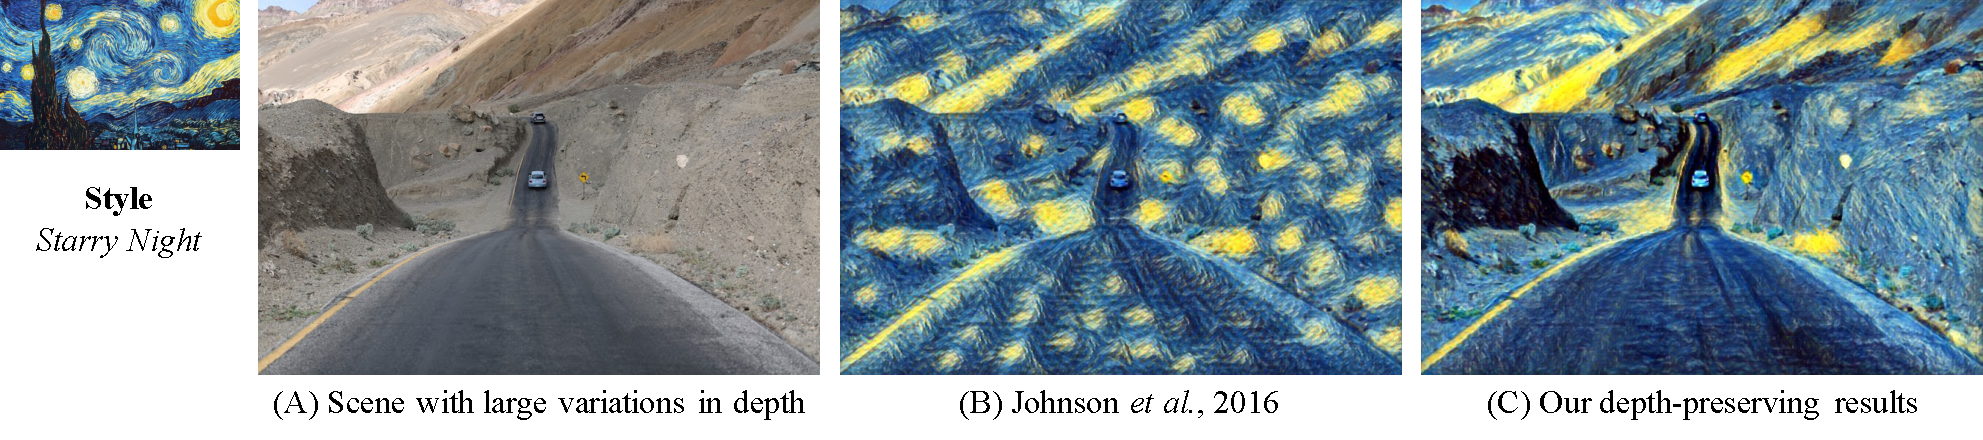
\includegraphics[width=\linewidth]{results/teaser.pdf}
When the input scene exhibits large variations in depth (A), the current state of the art tends to destroy the layering and lose the depth variations, producing a ``flat'' stylization result (B). This paper aims to address this issue by incorporating depth preservation into the loss function such that variations in depth and layering are preserved in the stylized image (C). 
\bigskip}
\makeatother

\maketitle
%\thispagestyle{empty}

%%%%%%%%% ABSTRACT
\begin{abstract}
   Style transfer is defined as the process that given a content image and a style image it tries to migrate the style from the style image to the content image. Though it is not clear what the exact definition of style is, pattern transforming and matching are generally accepted.

   In this work we present a novel method which preserve the depth information of the content image while migrating the style.
\end{abstract}

%%%%%%%%% BODY TEXT

\section{Introduction}

convolutional neural network (CNN)

\section{Related Work}

The core of our method is incorporating depth preservation losses into the image transformation neural network. Therefore, we review related literature on both neural network-based image style transfer and single-image depth estimation.

\subsection{Image Style Transfer with Neural Networks}

Style transfer can be considered as a more general form of texture transfer, where one transfers texture from one image (style image) to another image (content image). Ideally, semantics of the content image should not be altered in this process. In texture transfer, it is usually the low-level features that are utilized, \eg, in~\cite{efros2001image}.

With the recent prevalence of deep neural networks, researchers started exploring how high-level features extracted by neural networks can be utilized for the task of style transfer. For instance, Gatys \etal perform image style transfer by synthesizing a new image that matches both contents of the content image and styles of the style image~\cite{gatys2016image}. In particular, they extract content representations from the content image and style representations from the style image using the VGG network~\cite{simonyan2014very}. Since the VGG network is trained to perform object recognition and localization tasks, the layers deep down the network hierarchy capture object information (i.e., the contents) of the content image and are insensitive to the exact pixel values. Therefore, outputs from these deep layers serve as good content targets that the synthesized image tries to achieve at varying levels of resolution. As for style, they adopt a feature space built on filter responses in any layer of the network~\cite{gatys2015texture}. By design, the feature space captures texture information without global arrangement. Finally, they minimize a weighted sum of the content and style loss under a CNN framework, where forward and backward passes are iteratively performed. Building upon this work, the authors recently devised a way of preserve the original colors in the content image~\cite{gatys2016preserving}. However, the high computational cost still remains as a drawback in~\cite{gatys2016image}.

To reduce the computational burden and generate visually similar-quality results, Johnson \etal~\cite{johnson2016perceptual} train a feed-forward image transform network to approximate solutions to the optimization problem posed in~\cite{gatys2016image}. In particular, their system consists of a deep residual CNN as the image transform network and the pretrained VGG network~\cite{simonyan2014very} as the fixed loss network. For each style image, the image transform network is trained to apply this style to a content image while minimizing the style and content losses as measured by the loss network. This method produces reasonably good results with low computational cost, but tends to lose the depth variations and destroy layering in the content image as illustrated in the teaser figure. This issue can be addressed by incorporating depth preservation losses into the loss function, as shown later in this paper.

\subsection{Single-Image Depth Estimation}

Deep neural networks trained on ground-truth metric depth data have demonstrated promises in the task of single-image depth estimation~\cite{liu2015deep,eigen2015predicting,li2015depth,wang2015towards}. Collecting such ground truth requires specialized cameras, such as Kinect, posing a challenge to large-scale data collections. Although crowdsourcing may seem to be a solution, humans are known bad at estimating absolute depths (which are inherently ambiguous from a single monocular image), but better at at judging relative depths~\cite{todd2003visual}. Inspired by this fact, Zoran \etal train a neural network to repeatedly judge relative depths of point pairs and interpolate out per-pixel metric depth by solving an optimization problem~\cite{zoran2015learning}.

Building on~\cite{zoran2015learning}, a recent work by Chen \etal proposes an end-to-end neural network that takes in a single RGB image in the wild (\ie, taken in unconstrained settings) and outputs pixel-wise depth estimations~\cite{chen2016single}. Specifically, the deep network follows the ``hourglass architecture'' recently proposed in~\cite{newell2016stacked}, which is essentially a series of convolutions and downsampling followed by a series of convolutions and upsampling. Similar to~\cite{zoran2015learning}, RGB images with relative depth annotations are used as training data. The loss function penalizes large differences in metric depth when the ground-truth relative depth is annotated equal.

\section{Methods}

\begin{figure*}[h]
\centering
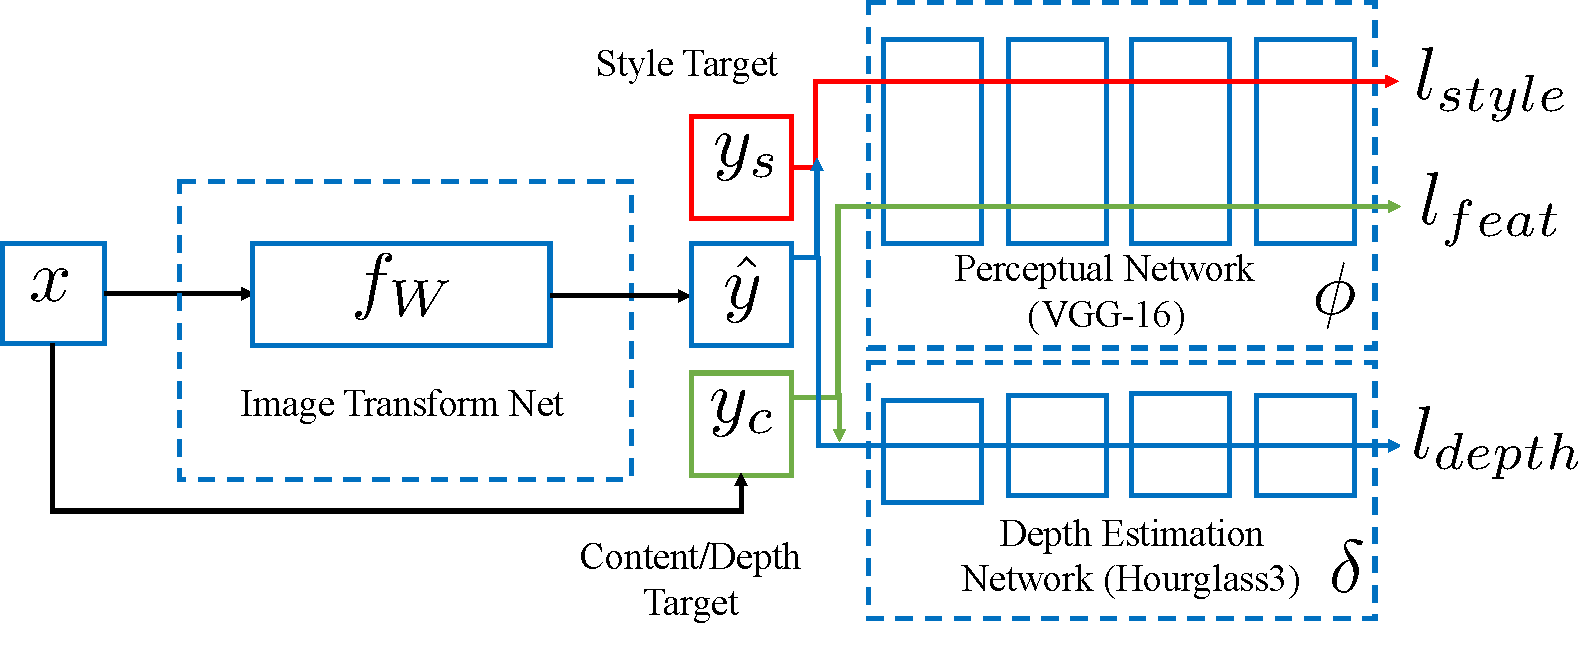
\includegraphics[scale=0.4]{network_structure.pdf}
\caption{Network Structure Overview}
\label{fig:overview}
\end{figure*}
The overview of our network structure is shown in Figure~\ref{fig:overview}. Compared to Johnson et al. \cite{johnson2016perceptual}'s work, our structure is featured in having a depth estimation network as part of our loss function. In all, our network is composed of 3 subnets: an image transformation network, a perceptual loss network and a depth estimation network. Similar to Johnson et al., the image transformation $f_W$ is a convolutional network which produce the output image $\hat y$ given the input image $x$ by $\hat y = f_W(x)$ (where $W$ is the weights of the network).

To keep track of the depth information, our loss function is composed of 2 neural networks: the perceptual loss network and the depth estimation network. As mentioned in \cite{johnson2016perceptual}, pretrained convolutional neural networks are able to extract perceptual information and encode semantics which are useful for the loss function. Similarly, a pretrained depth estimation network has already learned to estimate the depth information from the single input image. Therefore we utilize a pre-trained image classification network for the perceptual loss part and a pretrained depth estimation network for the depth loss part. Specifically, our loss function is defined as a weighted linear combination of the content loss $l_\text{content}$, the style loss $l_\text{style}$ and the depth loss $l_\text{depth}$. 

\[L(\hat y, y) = \lambda_1 l_\text{content}(\hat y, y) + \lambda_2 l_\text{style}(\hat y, y) + \lambda_3 l_\text{depth}(\hat y, y)\]

Therefore the training goal is to minimize the expected loss.

\[ W^* \gets \arg \min_W \mathbb E_{\{x,y\}}[L(f_W(x), y)], \]

where $\mathbb E_{\{x,y\}}$ is the estimation of the expectation via the (training) set $\{x,y\}$.

\subsection{Depth Loss Function}

We make use of depth loss function to quantify the amount of depth information preserved. 

\subsection{Content Feature Loss Function}

\subsection{Perceptual Style Loss Function}

\section{Experiments}

\section{Discussion \& Conclusion}



{\small
\bibliographystyle{ieee}
\bibliography{egbib}
}

\end{document}
